% Figure: the admissible cone. Referenced from §7 after rem:gaussian-extreme. Pure TikZ, on the
% design of Paper I's fig-admissible-cone, redrawn for this article's cone and for what THIS
% paper shows: the Gaussian ray as an extreme ray (rem:gaussian-extreme), the Cin rays on the
% far boundary (Appendix A exhibits them; that they are the other extreme rays is outside the
% paper and the caption says so), the stable exponents as the semigroup slice
% (cor:semigroup-case), the Matern ray (Appendix A). No Thorin region, no collar.

\begin{figure}[t]
\centering
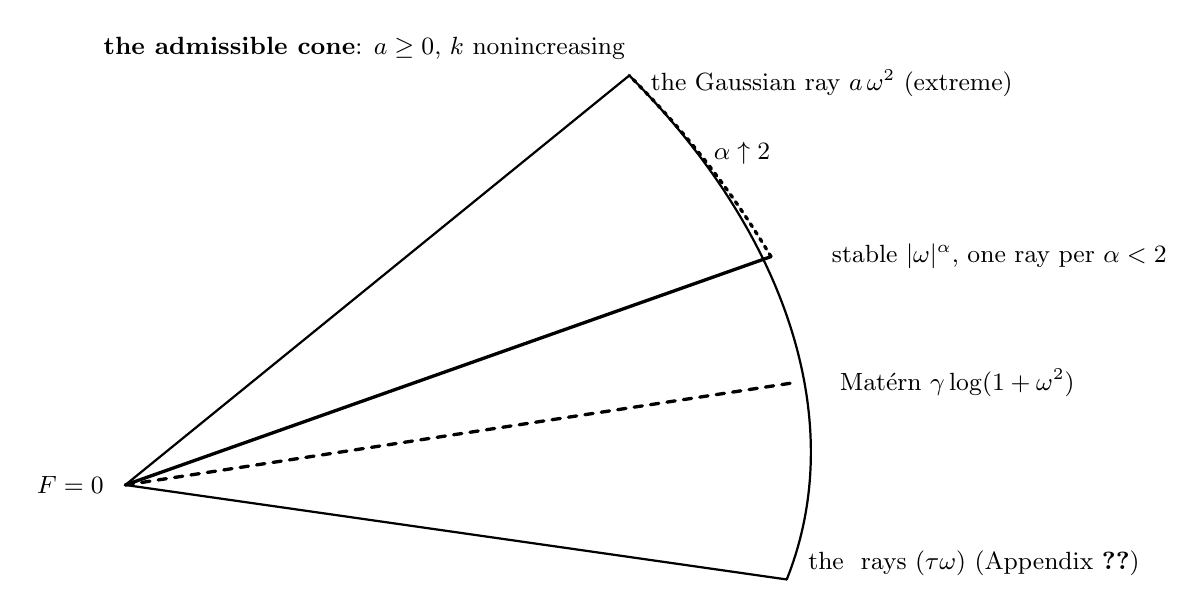
\begin{tikzpicture}[every node/.style={font=\small}, line cap=round, >=stealth]

% the cone, a wedge from the apex F = 0
\coordinate (O) at (0,0);
\draw[thick] (O) -- (6.4,5.2);     % upper edge: the Gaussian ray a omega^2
\draw[thick] (O) -- (8.4,-1.2);    % lower edge: a Cin ray
\draw[thick] (6.4,5.2) .. controls (8.4,3.2) and (9.2,0.8) .. (8.4,-1.2); % the far boundary: the Cin rays
\node[anchor=west] at (6.55,5.1) {the Gaussian ray $a\,\omega^2$ (extreme)};
\node[anchor=west] at (8.55,-1.0) {the $\Cin$ rays $\Cin(\tau\omega)$ (Appendix~\ref{sec:appendix})};
\node[anchor=east] at (-0.15,0) {$F = 0$};
\node[anchor=west] at (-0.4,5.55) {\textbf{the admissible cone}: $a \ge 0$, $k$ nonincreasing};

% the semigroup slice: the stable exponents, a curve of rays from alpha -> 0 to alpha = 2
\draw[very thick] (O) -- (8.2,2.9);
\node[anchor=west] at (8.85,2.9) {stable $|\omega|^{\alpha}$, one ray per $\alpha < 2$};
\draw[very thick,dotted] (8.2,2.9) .. controls (7.6,3.9) and (7.0,4.6) .. (6.4,5.2);
\node[anchor=south west] at (7.35,3.95) {$\alpha \uparrow 2$};
% the Matern ray
\draw[very thick,dashed] (O) -- (8.5,1.3);
\node[anchor=west] at (8.95,1.3) {Mat\'ern $\gamma\log(1+\omega^2)$};

\end{tikzpicture}
\caption{The admissible cone. Theorem~\ref{thm:main-characterization} identifies the
exponents $F$ with pairs $(a,k)$, a Gaussian coefficient and a nonincreasing profile, and
these form a convex cone (Lemma~\ref{lem:admissible-cone}). The Gaussian ray is an extreme
ray (Remark~\ref{rem:gaussian-extreme}), and it is a smoothing member, not a
degenerate boundary. The exponents of the unit-step profiles, the $\Cin$ rays of
Appendix~\ref{sec:appendix}, are the rays that generate the cone together with the Gaussian
ray: every admissible exponent is a superposition of them
(\ref{eq:cone-superposition}). They are drawn along the far side only to keep them apart;
whether they are extreme, which the superposition alone does not show, is outside this
paper, and the drawing places nothing. The semigroup case cuts the
slice of stable exponents $|\omega|^\alpha$ (Corollary~\ref{cor:semigroup-case}), one ray
for each $\alpha \in (0,2)$, and the slice ends on the Gaussian ray at $\alpha = 2$. The
Mat\'ern member of \S\ref{sec:axioms} is one ray, with the profile $2\gamma e^{-x}$
(Proposition~\ref{prop:matern-exponent}). The drawing is schematic: the cone is
infinite-dimensional.}
\label{fig:admissible-cone}
\end{figure}
